A base de dados em questão será usada para realização de tarefa de classificação segundo o paradigma de aprendizado supervisionado. Nesta tarefa, exemplos de expressões faciais e seus respectivos rótulos serão fornecidos previamente aos modelos de Aprendizado de Máquina para escolha e ajuste de parâmetros e realização do treinamento. Posteriormente, expressões faciais ainda não vistas serão apresentadas e o objetivo será avaliar o desempenho do modelo na classificação destes exemplos, isto é, aferir a respectiva capacidade de generalização.

Obedecendo a uma partição do FER2013 previamente considerada em competições de Visão Computacional \cite{Kaggle:FER2013}, esta base de dados será dividida em $3$ partes, sendo: $75\%$ dos exemplos para treinamento (partição \emph{Training}), e $25\%$ dos dados para testes, segundo uma abordagem \emph{holdout} de validação cruzada \cite{Brink:MachineLearningLivro}.  Do conjunto de testes, metade do mesmo será utilizada livremente (partição \emph{Public Test}), mas a outra metade (partição \emph{Private Test}, cerca de $1/8$ da base de dados original) será utilizada para obtenção das métricas de desempenho e comparação dos modelos. Conforme ilustra a Figura \ref{fig:particoes}, as partições preservam a distribuição de amostras por classe na base de dados original.

\begin{figure}[h!]
	\centering
  	\caption{Distribuição das classes nas partições adotadas para o conjunto de dados.} \label{fig:particoes}
	\subfloat[\emph{Training}]{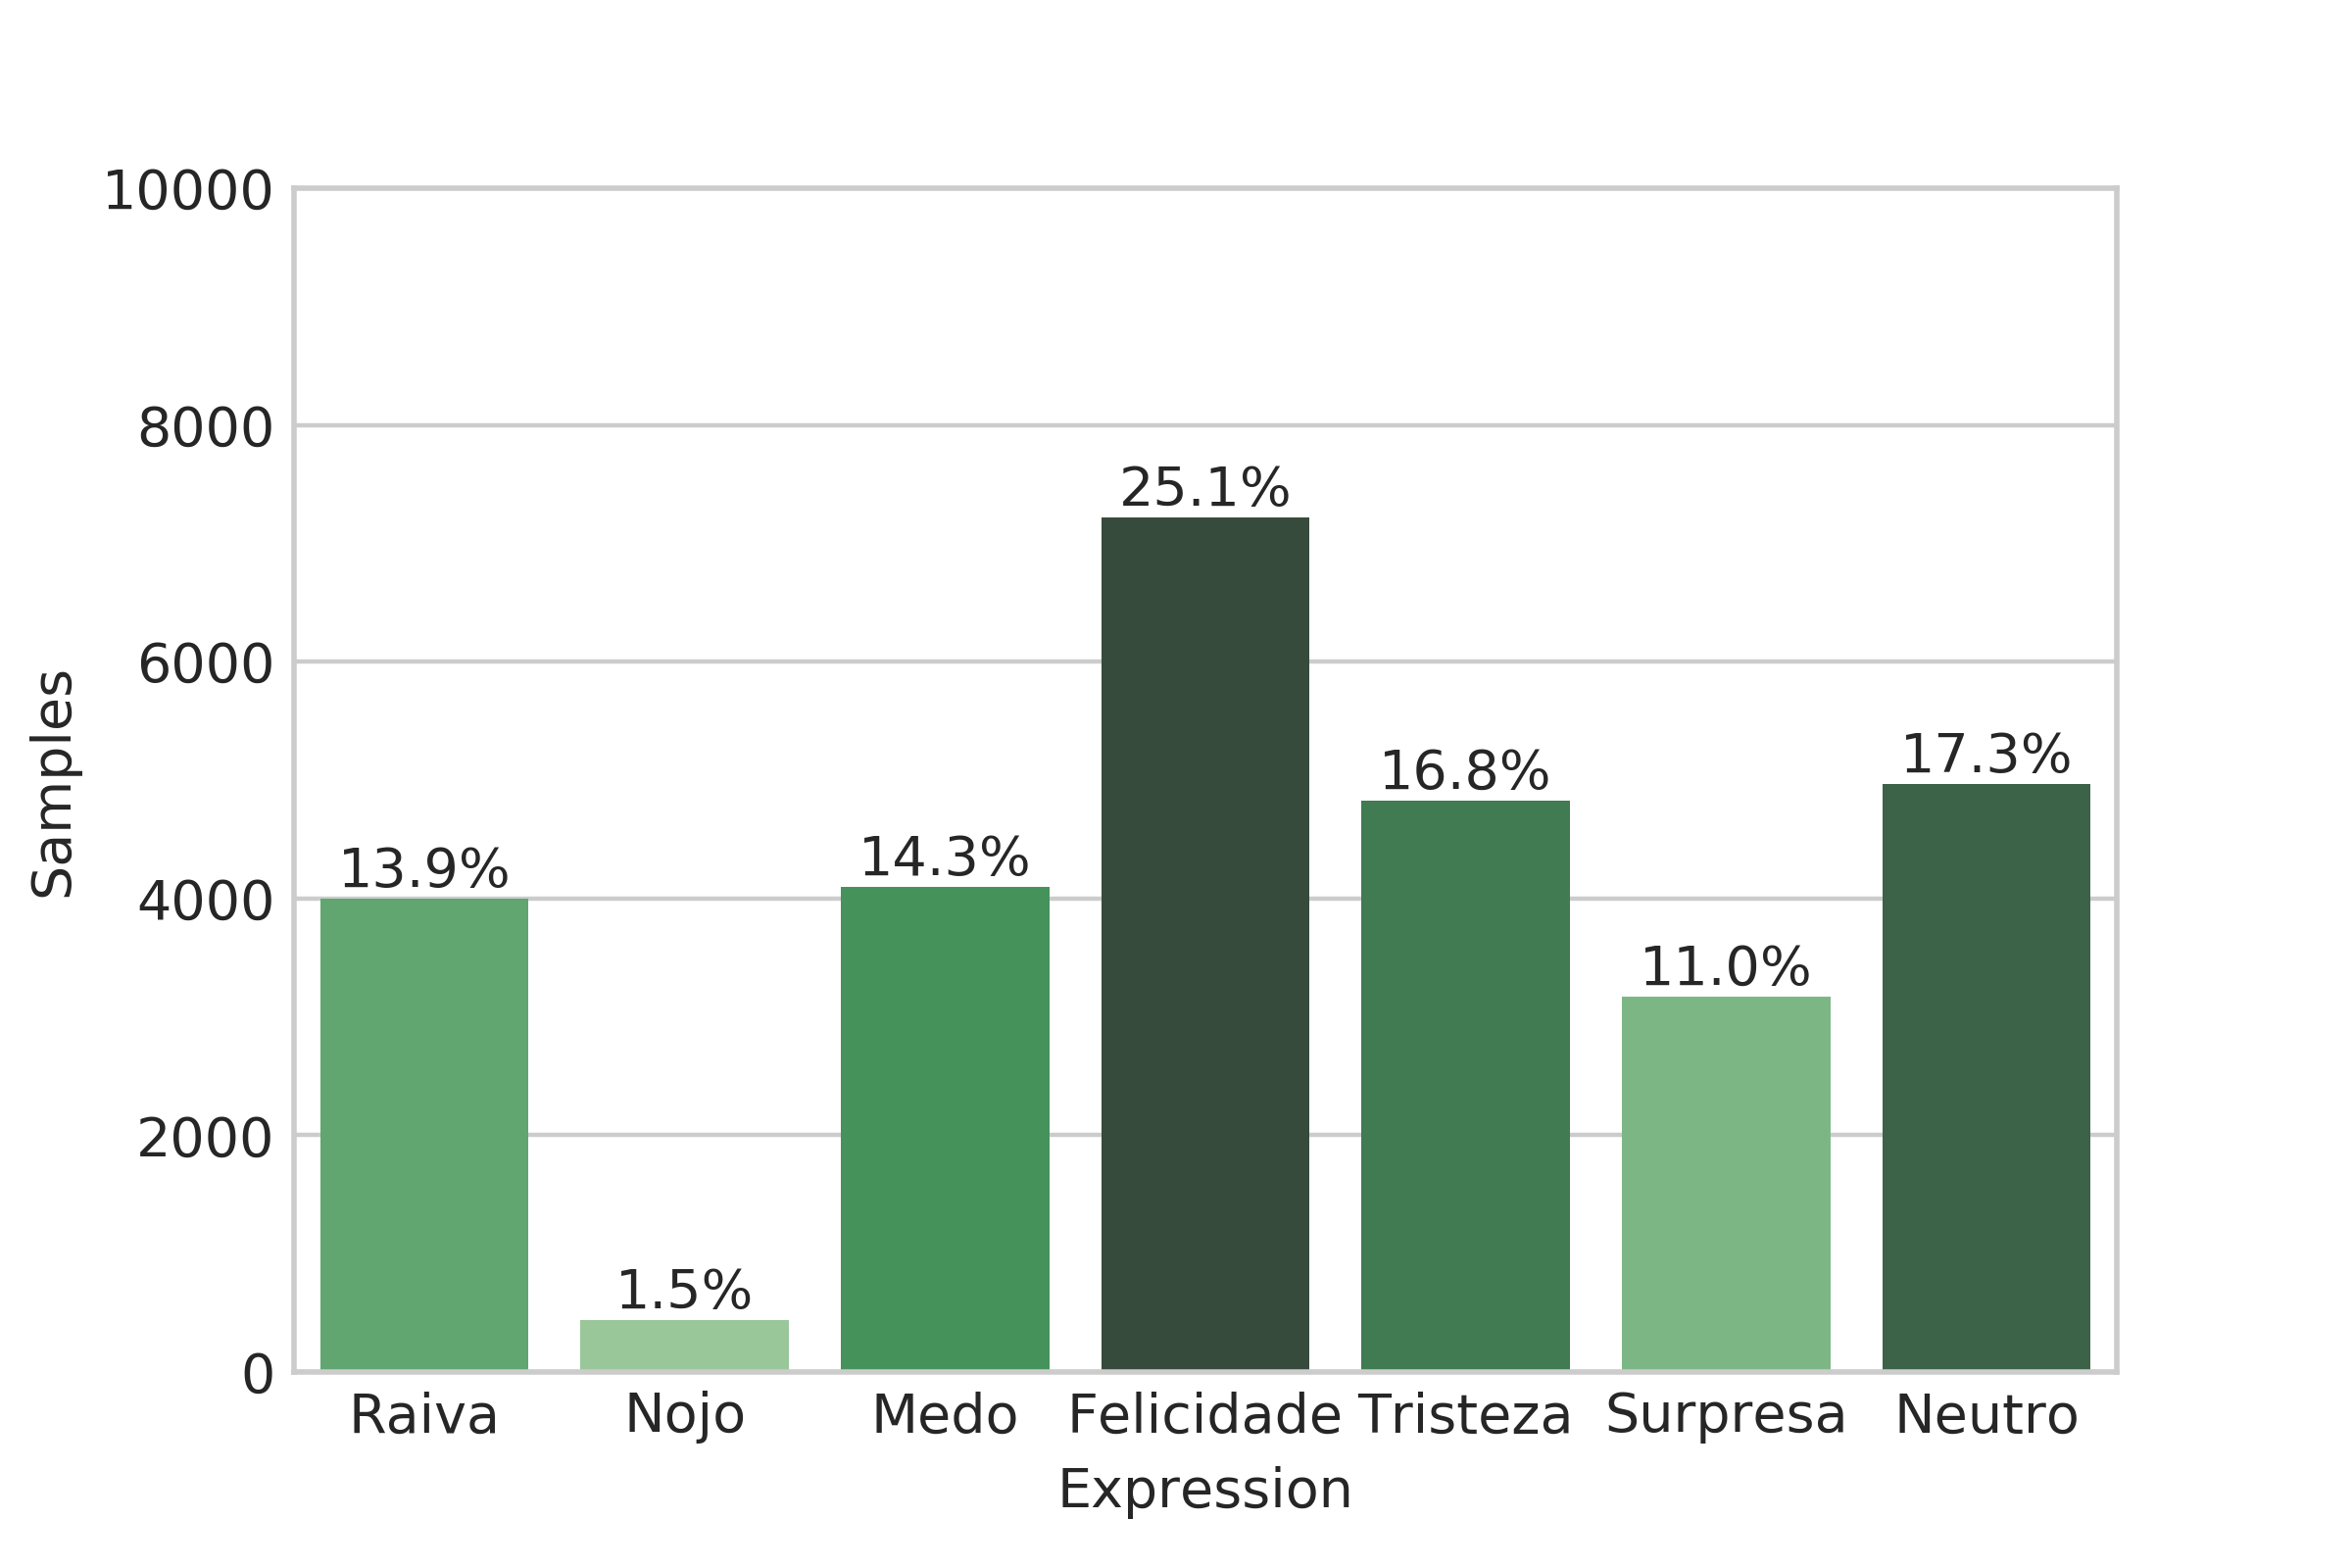
\includegraphics[width=0.3\linewidth]{images/expression_distribution_training.png}}
	\subfloat[\emph{Public Test}]{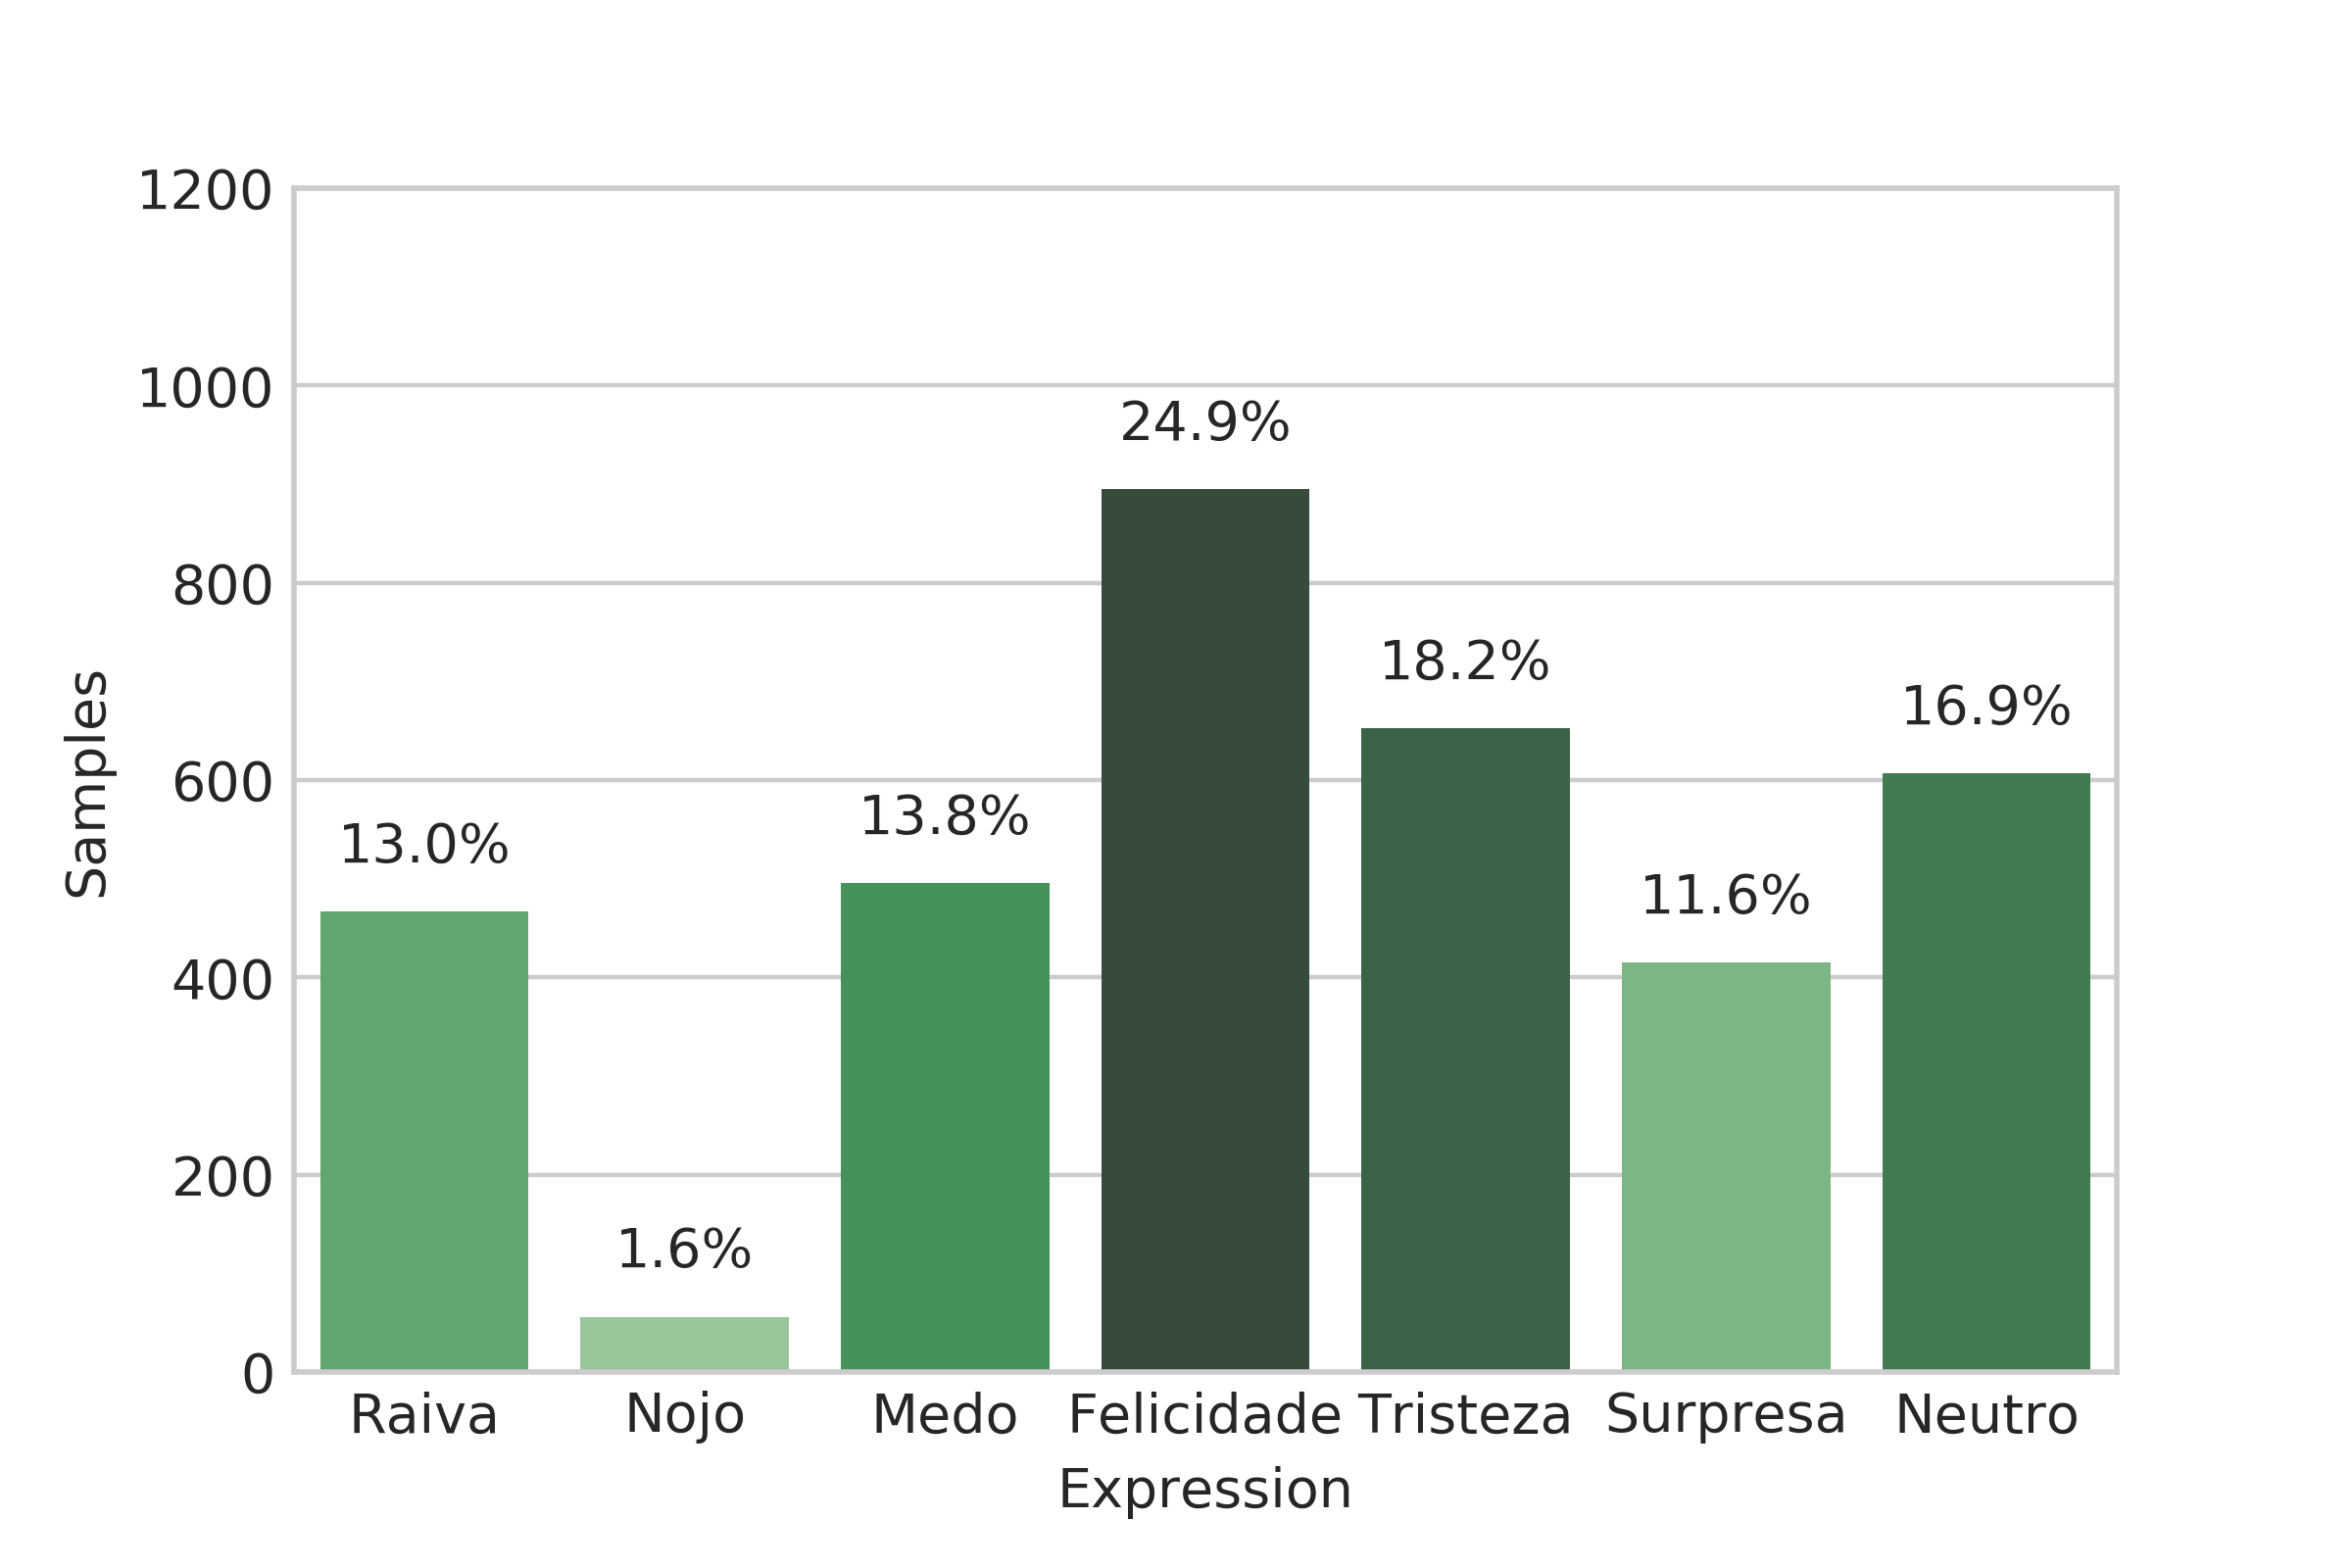
\includegraphics[width=0.3\linewidth]{images/expression_distribution_validation.png}}
	\subfloat[\emph{Private Test}.]{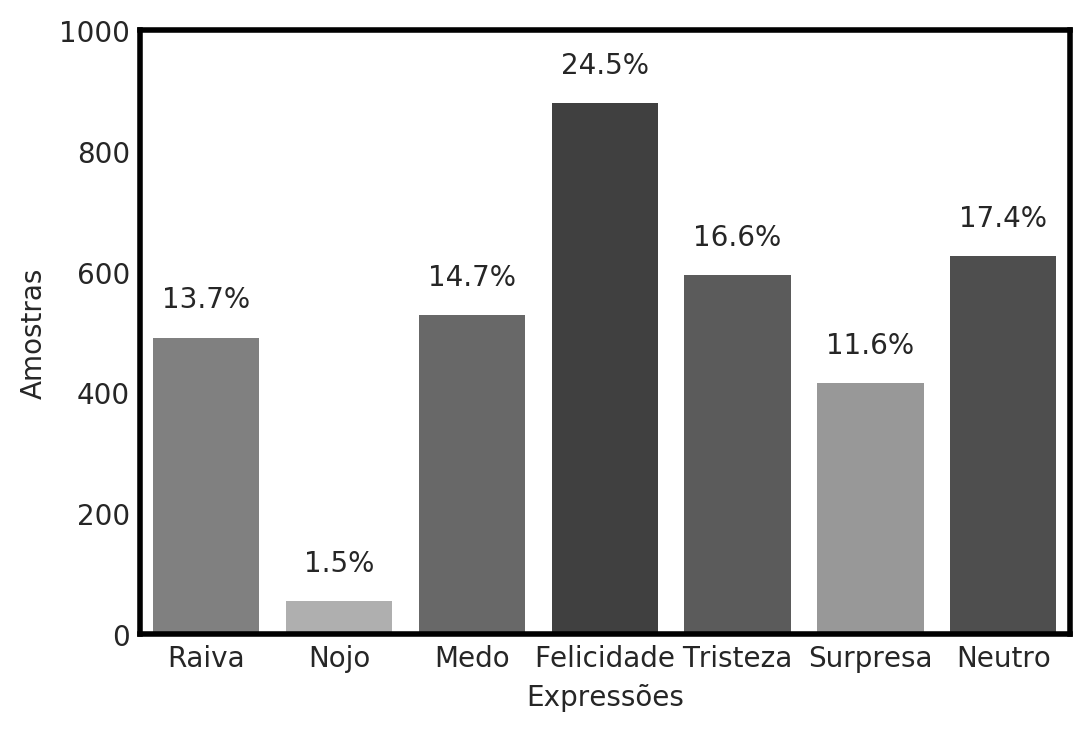
\includegraphics[width=0.3\linewidth]{images/expression_distribution_test.png}}
\end{figure}

Duas métricas de desempenho serão utilizadas para comparação dos modelos na realização desta tarefa: a acurácia e o Micro $F$-\emph{Score}. A acurácia é uma métrica intuitiva que descreve o percentual de acertos do modelo em relação ao total de previsões efetuadas. Embora forneça uma visão geral da capacidade de generalização do modelo, não fornece detalhes acerca dos acertos por classe. Para contornar esta dificuldade, o Micro $F$-\emph{Score} também será utilizado, pois contempla a média harmônica entre precisão e revocação por classe ao passo que considera as diferentes frequências nas classes do problema \cite{Kubat:Livro}. Esta métrica é comumente utilizada em problemas de classificação com classes desbalanceadas, similar ao cenário considerado no escopo deste trabalho.

Dentre os modelos a serem avaliados, serão elencados como mais aptos para a tarefa considerada aqueles que maximizarem as duas métricas de desempenho para os exemplos pertencentes à partição \emph{Private Test}.






% Desnecessário: confuso!
%Para validação do \emph{XGBoost} foi utilizado a validação cruzada estratificada \cite{}, para que o desbalanceamento das classes na base de dados fosse replicada nas partições. O número de partições recomendado pela literatura é dez \cite{}, contudo, este valor é sugerido para base de dados grandes, o que não reflete a realidade da escolhida. Para a validação deste modelo foi escolhido sete partições, pois, o conjunto \emph{PrivateTest} é aproximadamente $\frac{1}{8}$ da base de dados, o que deixa $\frac{7}{8}$ a serem divididos na validação cruzada. Ressaltando que o conjunto \emph{PrivateTest} foi mantido fixo e utilizado somente como validação final do modelo, para que a comparação com os resultados da competição no \emph{Kaggle} fosse realizada.
